\documentclass[11pt,twoside,openany,svgnames,x11names]{gkbookm1}
%%%%%%%%%%%%%%%%%%%%%%%%%%%%%%%%%%%%%%%%%%%%%%%%%%%%%%%%%%%%%%%%%%%%%
%\fcolorbox{declared-color-frame}{declared-color-background}{text}
\setlength{\parindent}{0pt}  % or \usepackage{parskip} \parskip

\begin{document}
\frontmatter %% Cover page %%%%%%%%%%%%%%
\thispagestyle{empty}  %% No header footer
\ThisCenterWallPaper{0.85}{clw1.jpg} %WheelRITES.png} %
\tikz[remember picture,overlay]%
\node[fill=Sienna,text=white,font=\LARGE\bfseries,text=Cornsilk,%
minimum width=\paperwidth,minimum height=5em,anchor=north]%
at (current page.north){Offer No: WA/CLW/eLocomotives/0001{ }\today};

{\centering \bfseries\color{LightGoldenrod!40!blue}\fontsize{32pt}{46pt}\selectfont Indian Railways Standard \par Electric Locomotives %\\ Chittaranjan Locomotive Works, Chittaranjan
	\par }

\vspace*{32\baselineskip}
\begin{center}
{\LARGE\color{blue} \textbf{  \scshape{Indian Railways and RITES} } \par  }   % LightGoldenrod}
\end{center}

\tikz[remember picture,overlay]%
\node[fill=Sienna,font=\LARGE\bfseries,text=Cornsilk,
minimum width=\paperwidth,minimum height=3em,anchor=south]at (current page.south)%{One Line Text};
{Expotech Division, RITES Limited, India};

\begin{center}
\LARGE\bfseries\color{SaddleBrown!30!black}
RITES proposal for supply of Standard Gauge Electric Locomotives
\end{center}

%%%%%%%%%%%%%%%%%%%%%%%%%%%%%%%%%%%%%%%%%%%%%%%%%%%%%%%%%%%%%%%%%%%%%%%%%%%%%%%%%%%%%%%%%%%%%%%%%%%
%%%%%%%%%%%%%%%%%%%%%%%%%%%%%%%%%%%%%%%%%%%%%%%%%%%%%%%%%%%%%%%%%%%%%%%%%%%%%%%%%%%%%%%%%%%%%%%%%%
\newpage
%COPYRIGHT PAGE%-
\thispagestyle{empty}
\begin{center}
\includegraphics[scale=0.35]{RITESbuilding1.jpg} %logo}
\end{center}

%~\vfill
\vskip 2cm

\noindent 

\begin{center}
\begin{tikzpicture}    % Now typeset a sample box.
\node[text width=.5\textwidth,   fill=yellow!30,   fill opacity=0.6,  text opacity=0.8,   	%but this also makes photo transparent
      inner sep=10pt]{	 \centering {\bf\Large A Government of India Compnay \\ under Ministry of Railways}\\
      Chittaranjan Locomotive Works \\
\vskip 0.3cm   
   \includegraphics[width=0.5\textwidth]{RITESlogo} \\
\vskip 0.4cm
}; %Photo insertion credit: gopalkumar@rites.com   };
\end{tikzpicture}

\end{center}


\vfill

%\AddToShipoutPicture*{ \put(150,50){  \includegraphics[scale=0.24]{RITESlogo.png}  } } % bottom Image background


\begin{center}
%\colorbox{white}{\EANisbn[SC4]}
\includegraphics[scale=0.551]{img/gkqrcode.jpg}

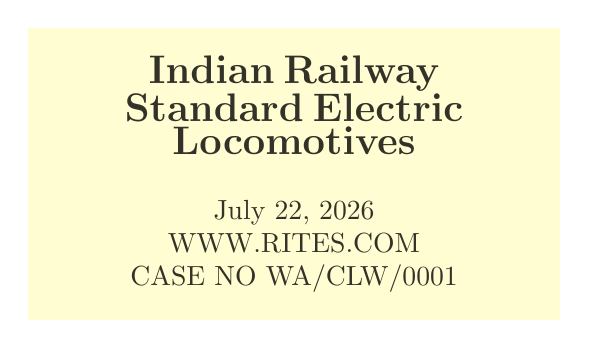
\begin{tikzpicture}    % Now typeset a sample box.
\node[text width=.5\textwidth,   fill=yellow!30,   fill opacity=0.6,  text opacity=0.8,   inner sep=10pt]  	%but this also makes photo transparent
    {	 \centering {\bf\Large Indian Railway Standard Electric Locomotives}\\
\vskip 0.4cm
\today \\
WWW.RITES.COM\\
CASE NO WA/CLW/0001\\
};
\end{tikzpicture}

\vspace*{\baselineskip}

\textbf{\textcolor{red!80}{Expotech Division, RITES Limited \texttt{http://www.rites.com}}}
\vspace*{\baselineskip}

\colorbox{white}{
\textbf{\textcolor{red!60}{Cover Illustration: Indian Railway Locomotives  \textbullet\ \texttt{http://www.rites.com}}}   }
\end{center}


\noindent Copyright \copyright\ RITES Ltd 2016\\ % Copyright notice

\noindent \textsc{Expotech Division}\\ % Publisher

\noindent \textsc{www.rites.com}\\ % URL

\noindent This offer is prepared for the specific use of RITES prospective clients to enable technical and commercial evaluation of the offer submitted by RITES.
For any clarification, please contact gopalkumar@rites.com  \url{http://www.rites.com}.\\ % License information

\noindent \textit{ \today} % Printing/edition date



%%%%%%%%%%%%%%%%%%%%%%%%%%%%%%%%%%%%%%%%%%%%%%%%%%%%%%%%%%%%%%%%%%%%%%%%%%%%%%%%%%%%%%%%%%%%%%%%%%%
\cleardoublepage
\tableofcontents
%%%%%%%%%%%%%%%%%%%%%%%%%%%%%%%%%%%%%%%%%%%%%%%%%%%%%%%%%%%%%%%%%%%%%%%%%%%%%%%%%%%%%%%%%%%%%%%%%%%
\mainmatter%startarabic1
\pagestyle{headings}

%%%%%%%%%%%%%%%%%%%%%%%%%%%%%%%%%%%%%%%%%%%%%%%%%%%%%%%%%%%%%%%%%%%%%%%%%%%%%%%%%%%%%%%%%%%%%%%%%%%
%\input{chp/CLWStickyNotes.tex}
%%%%%%%%%%%%%%%%%%%%%%%%%%%%%%%%%%%%%%%%%%%%%%%%%%%%%%%%%%%%%%%%%%%%%%%%%%%%%%%%%%%%%%%%%%%%%%%%%%%

%%%%%%%%%%%%%%%%%%%%%%%%%%%%%%%%%%%%%%%%%%%%%%%%%%%%%%%%%%%%%%%%%%%%%%%%%%%%%%%%%%%%%%%%%%%%%%%%%%%
%\chapter{Introduction \& Background}  %get belownoted image
%\renewcommand\chapterillustration{img/WheelRITES.png} %WheelFurnace.jpg}
%\input{chp/KRCintro.tex}  %Add if useful \ClientICSWho,
%%%%%%%%%%%%%%%%%%%%%%%%%%%%%%%%%%%%%%%%%%%%%%%%%%%%%%%%%%%%%%%%%%%%%%%%%%%%%%%%%%%%%%%%%%%%%%%%%%%


%%%%%%%%%%%%%%%%%%%%%%%%%%%%%%%%%%%%%%%%%%%%%%%%%%%%%%%%%%%%%%%%%%%%%%%%%%%%%%%%%%%%%%%%%%%%%%%%%%%
\chapter{Electric Locomotives from Indian Railways}
\renewcommand\chapterillustration{img/IRlogo.jpg}
\section{The Indian Railways Locomotive manufacturing}

CLW manufactures Electric Locomotives for captive use over the Indian Railways Network of over 100 thousand track kilometres. it is one of the largest Electric Locomotive manufacturer in the world.   


The production activity started on 26th January, 1950 the day when India became Republic. Chittaranjan Locomotive Works (CLW) has been named after the great freedom fighter, leader and statesmen Deshbandhu Chittaranjan Das .
 The initial product of Chittaranjan Locomotive Works was Steam Locomotive. In the period 1950-1972 Chittaranjan Locomotive Works turned out a total number of 2351 Steam Locomotives.


The locomotives profile ranges includes three phase ac drive, 25kv ac locomotive with dc drive. 


CLW also manufactures AC \& DC Traction motors, Switch gears/Control gears, Bogies cast \& fabricated, Wheel sets \& Steel casting.


%At a glance information of Rail Wheel Factory at Bangalore in India.


\begin{tabular}[h]{|l|p{3cm}|}
Land   Acquired  &  291 acres \\
Land for workshop & 191 acres \\
Land for colonies & 100 acres \\
Cost of 291 acres of land & 14.55 lakhs \\
Annual Turn Over & 1094 crores.\\
Direct employees & 2600 \\
Railway track &  16 kms. \\
No. of Quarters &  940 \\
Treasure of trees & More than 43000 trees\\
Water consumption per day & 16.13 lakh Litres \\
Power  & \\
Connected Load & 90MVA \\
Average consumption per month & 28MVA \\

Initial plant  capacity  &  56,700 wheels\\
                        & 23000 axles \\
                        & 23000 wheelsets \\
Present capacity & \\ 
					& 1,90,000 wheels;\\
					& 70,00 axles \\
					& 59,640 wheelsets \\
Quality Management System & ISO 9001:2008 \\
Environment Management System & ISO 14000:2004 \\
Occupational Health and Safety system & OHSAS 18001:2007 \\
manufacture of wheels &
Bottom pouring casting technology \\
Manufacturing of Axles & Radial Forging Technology \\
\end{tabular}





\section{The Electric Locomotives from CLW}

\begin{center}
\includegraphics[ width=0.8\textwidth]{img/clwlocos12.jpg}
\end{center}

\section{The Traction Motors form CLW}
\begin{center}
\includegraphics[ width=0.8\textwidth]{img/clwmotor.jpg}
\end{center}


%%%%%%%%%%%%%%%%%%%%%%%%%%%%%%%%%%%%%%%%%%%%%%%%%%%%%%%%%%%%%%%%%%%%%%%%%%%%%%%%%%%%%%%%%%%%%%%%%
\cleardoublepage
%\chapter[Product Range of Wheel and Axles]{Product Range of Wheel and Axles}
%\renewcommand\chapterillustration{img/IRlogo.jpg}
%\section{RWF current product range on offer}

Major portion of the product of Rail Wheel Factor is consumed in house by the Indian Railway.
RWF has improved its productivity to offer the following quality products at the low overheads at the competitive rates.

\section{The Wheel Disks}

%\begin{figure}[Ht]
\begin{center}
\includegraphics[width=00.40\linewidth, angle=0]{img/RWFwheelFEA1.png} \quad
\includegraphics[width=00.40\linewidth, angle=0]{img/RWFwheelFEA2.png}
%\caption{Loading parameters thermal load 25 HP Vertical. load: 21.5T Time: 20 min for both Forged and cast  EMU wheels}
\end{center}
%\end{figure}

\includegraphics[width=01.0\linewidth]{img/RWFwheelrange.jpg}




\section{The Axles}

\begin{center}
\includegraphics[width=00.60\linewidth, angle=0]{img/Axles2.jpg} 
\end{center}

\includegraphics[width=01.0\linewidth]{img/RWFaxlerange.jpg}




\section{The Wheelsets}

\includegraphics[width=01.0\linewidth]{img/RWFwheelsetsrange.jpg}

\section{The cast wheel specifications}

\begin{center}
	\includegraphics[width=0.8\linewidth, angle=-0]{../img/RWFSpecs.pdf} 
\end{center}


%\newpage
%At a glance information of Rail Wheel Factory at Bangalore in India.


\begin{tabular}[h]{|l|p{3cm}|}
Land   Acquired  &  291 acres \\
Land for workshop & 191 acres \\
Land for colonies & 100 acres \\
Cost of 291 acres of land & 14.55 lakhs \\
Annual Turn Over & 1094 crores.\\
Direct employees & 2600 \\
Railway track &  16 kms. \\
No. of Quarters &  940 \\
Treasure of trees & More than 43000 trees\\
Water consumption per day & 16.13 lakh Litres \\
Power  & \\
Connected Load & 90MVA \\
Average consumption per month & 28MVA \\

Initial plant  capacity  &  56,700 wheels\\
                        & 23000 axles \\
                        & 23000 wheelsets \\
Present capacity & \\ 
					& 1,90,000 wheels;\\
					& 70,00 axles \\
					& 59,640 wheelsets \\
Quality Management System & ISO 9001:2008 \\
Environment Management System & ISO 14000:2004 \\
Occupational Health and Safety system & OHSAS 18001:2007 \\
manufacture of wheels &
Bottom pouring casting technology \\
Manufacturing of Axles & Radial Forging Technology \\
\end{tabular}



\section{Technical Specification of Electric Loco's}



\includepdf[pages={1,2,3}, frame, scale=0.8,%landscape %nup=2x2, deltax=10, deltay=10, %
pagecommand={\thispagestyle{plain}}  ]
{img/eLocos.pdf}


% % % % % % % % % % % % % % % % %
%\renewcommand\chapterillustration{img/WheelRITES.png}%\chapter{Appendix}
%\clearpage 
%\pagestyle{fancy}
%\section*{ Copy of the KRC invitation for EOI}
%\pagestyle{fancy}
%\pagenumbering{num_style} %arabic:roman:Roman:alph: Alph: 

%\includegraphics[ scale=0.8]{chp/KRCsafetyEOI.pdf} % try \includepdf[scale=0.8,pages=1,pagecommand=\subsection{blub}]{testpdf}

% % % % %was OK but page number not coming
%\includepdf[ pages={1,2,3,4,5,6,7,8,9,10}, nup=2x2, %landscape,    %pages={1,{}, 4-6,9 } , % , landscape, linktodoc]
%frame, scale=0.80, %trim = 10mm 80mm 20mm 5mm, clip,
%deltax=10, deltay=10, %page separation
%offset=0 0 %Displace the origin of the included pages
%angle=-0, offset=0in 0in,    
%addtolist={3, table, {The User Roles table}, tab:UserRoles}, 
%pagecommand={} %{\pagestyle{fancy}} %plain}} %headings}} %plain}}
%]{chp/KRCsafetyEOI.pdf}
% % % % % % % % % % % % % % % % % % %
%\chapter[The Rail Wheel Factory]{Rail Wheel Factory}
%\renewcommand\chapterillustration{img/WheelRITES.png}


\includepdf[pages={1}, frame, scale=0.75,%landscape %nup=2x2, deltax=10, deltay=10, %
pagecommand={\thispagestyle{plain}}  ]
{img/clwlocos.jpg}


%%%%%%%%%%%%%%%%%%%%%%%%%%RITES
\chapter[The RITES limited]{The RITES limited}
\renewcommand\chapterillustration{img/RITESlogo3.jpg}
%\newpage
%\section{Capabilities of RITES in brief}
\section{RITES Limited}

\subsection{Background}

%\medskip

RITES Ltd., a Government of India Enterprise was established in 1974, under the aegis of Indian Railways. RITES is incorporated in India as a Public Limited Company under the Companies Act, 1956 and is governed by a Board of Directors which includes persons of eminence from various sectors of engineering and management.

RITES Ltd., an ISO 9001:2008 certified company, is a multi-disciplinary consultancy organization in the fields of transport, infrastructure and related technologies. It provides a comprehensive array of services under a single roof and believes n transfer of technology to client organizations. In overseas projects, RITES actively pursues and develops cooperative links with local consultants / firms, as means of maximum utilization of local resources and as an effective instrument of sharing its expertise.

RITES is internationally recognized as a leading consultant with operational experience of 62 countries in Africa, South East Asia, Middle East and Latin America. Most of RITES foreign assignments are for National Governments and other apex organizations.

\section{OUR RESOURCES}

RITES employs over 2000 staff including over 1200 specialists of high professional standing in the fields of engineering, management and planning. Besides full time professionals, RITES also has on its panel a large number of experts, whose services can be drawn upon at short notice. 
This provides the company unmatched strength in meeting the needs of its clients worldwide.



\section{Board of Directors}
\noindent

Mr. Rajeev Mehrotra , Chairman \& Managing Director\\

Mr. Arbind Kumar, Director Projects \\

Mr. Ajay Kumar Gaur, Director Finance \\

Mr. Shashi Bhushan Malik,  Director Technical \\

Mr. R. S. Kochak, Govt. Nominee Director \\

Mr. A P Dwivedi , Govt. Nominee Director   \\


{\color[rgb]{0.0,0.0,0.04}
Since the late sixties, Indian Railways have been extending technical co-operation to developing countries in the field
of railroad technology. These services made a start in Jordan and were later extended to other countries including
Iraq, Philippines, Saudi Arabia, Thailand, Iran, Ghana, Nigeria, Tanzania, Kenya, Ethiopia, Uganda, Mozambique, Sudan,
Zambia, Zimbabwe, Sri Lanka, Burma, Vietnam, Bangladesh and Mexico.}


\bigskip

{\color[rgb]{0.0,0.0,0.039215688}
With the increase in world-wide demand for professional services in various fields of transportation technology,
particularly in the context of expansion and modernization of existing transport systems, it became necessary to
channelize, on a rational basis, the export of technological know-how, expertise and special skills acquired by the
Indian Railways over the past 50 years or so. }


\bigskip

\subsection{Organization}

\bigskip

{\color[rgb]{0.0,0.0,0.039215688}
RITES Ltd, a Government of India Enterprise, was established in 1974. RITES Ltd. is incorporated in India as a Public
Limited Company under the companies Act, 1956 and is governed by Board of Directors, which includes experts/
administrators of eminence from various sectors of activities of RITES interest. }


\bigskip

{\color[rgb]{0.0,0.0,0.039215688}
RITES Ltd specializes in providing comprehensive consultancy services under a single roof and believes in sharing its
experience with client organizations. \ }


\bigskip

{\color[rgb]{0.0,0.0,0.039215688}
RITES Ltd, employs nearly 2000 staff including nearly 1200 specialists of high professional standing in the fields of
Engineering, Management, Planning and Financial analysis. Besides full time professionals, RITES Ltd., has on its panel
a large number of experts, whose services can be drawn at short notice. This provides the company an unmatched strength
in meeting the needs of the clients Worldwide.}


\section{Brief Introductory Brochure of RITES}
\includepdf[ pages={2,3,4,6,10,17,14,19,20,22,23,25,30,31,32}, frame, scale=0.880, %3}, frame, scale=0.880,  %
%nup=2x2, deltax=10, deltay=10, %
pagecommand={\thispagestyle{plain}}
]{chp/RITESBrochure2014.pdf} 

%\appendix

%\renewcommand\chapterillustration{img/WheelRITES.png} 
%\chapter{Appendix}
%\clearpage 
%\pagestyle{fancy}
%\section*{ Copy of the KRC invitation for EOI}
%\pagestyle{fancy}
%\pagenumbering{num_style} %arabic:roman:Roman:alph: Alph: 

%\includegraphics[ scale=0.8]{chp/KRCsafetyEOI.pdf} % try \includepdf[scale=0.8,pages=1,pagecommand=\subsection{blub}]{testpdf}

% % % % %was OK but page number not coming
%\includepdf[ pages={1,2,3,4,5,6,7,8,9,10}, nup=2x2, %landscape,    %pages={1,{}, 4-6,9 } , % , landscape, linktodoc]
%frame, scale=0.80, %trim = 10mm 80mm 20mm 5mm, clip,
%deltax=10, deltay=10, %page separation
%offset=0 0 %Displace the origin of the included pages
%angle=-0, offset=0in 0in,    
%addtolist={3, table, {The User Roles table}, tab:UserRoles}, 
%pagecommand={} %{\pagestyle{fancy}} %plain}} %headings}} %plain}}
%]{chp/KRCsafetyEOI.pdf}
% % % % % % % % % % % % % % % % % % %

% % %page of
%\includepdf[pages=-, nup=2x2,
%frame, scale=0.80,
%deltax=10, deltay=10,
%pagecommand={\thispagestyle{plain}}]{chp/KRCsafetyEOI.pdf}
%\includepdf[pages=-,frame,scale=0.85, nup=2x2,
%pagecommand={\pagestyle{plain}}]{chp/KRCsafetyEOI.pdf} %page numbers.

%\input{chp/KRCrequirements.tex} %text not corrected

%%%%%%%%%%%%%%%%%%%%%%%%%%%%%%%%%%%%%%%%%%%%%%%%%%%%%%%%%%%%%%%%%%%%%%%%%%%%%%%%%%%%%%%%%%%%%%%%%%%

%%%%%%%	    Colophon	%%%%%%%%%%%%%%%%%%%%%%%%%%%%%%%%%%%%%%%%%%%%%%%%%%%%%%%%%%%%%%%%%%%%%%%%%%%%%%
\clearpage
\pagestyle{empty}\newpage\mbox{This page is intentionally blank to enable quatro print}
%\clearpage

\begin{tikzpicture}[remember picture,overlay]  %%%%%%%%%%%for next page transperant text box
  \node[inner sep=0pt] at (current page.center) {  \includegraphics[width=\paperwidth,height=\paperheight] {TajMahal4.jpg}  };%
\end{tikzpicture}

\vskip -3.0cm
\begin{tikzpicture}     % Now typeset a sample box.
\node[textwidth=.5\textwidth, fill=blue!30, fill opacity=0.3, text opacity=0.7, inner sep=10pt]{
This booklet created using all 'Free Open Source Softwares (FOSS)' on Linux platform};
\end{tikzpicture}

\vspace*{\stretch{1}}
   % TajMahal with colophon one line text

%%%%%%%%	Back cover	%%%%%%%%%%%%%%%%%%%%%%%%%%%%%%%%%%%%%%%%%%%%%%%%%%%%%%%%%%%%%%%%%%%%%

%%%%%%%%%%%%%%%%%%%%%%%%%%%%%%%%%%%%%%%%%%%%%%%%%%%%%%%%%%%%%%%%%%%%%%%%%%%%%%%%%%%%%%%%%%%%%%%%%%%%%%%%
%%%%%%%%%%%%   Back Cover of the Book               %%%%%%%%%%%%%%%%%%%%%%%%%%%%%%%%%%%%%%%%%%%%%%%%%%%%%
\clearpage   
% Add a background image for the full page
\begin{tikzpicture}[remember picture,overlay]
\node[inner sep=0pt] at (current page.center) 
{\includegraphics[width=\paperwidth,height=\paperheight]{img/TajMahal4.jpg} };
\end{tikzpicture} %  Repeat same block for another image


%\noindent 

\begin{tikzpicture}     % Now typeset a sample box.
  \node[text width=.95\textwidth, fill=green!30, fill opacity=0.5, text opacity=1, inner sep=10pt]{
  {\bf\Large The Taj Mahal at Agra } \\
%  \lipsum[1]
The TajMahal is one of the world famous monoments in India , at Agra, near Delhi.\\ Contact at gopalkumar@rites.com for further details.\\

};
\end{tikzpicture}


\vspace*{\stretch{1}}


\begin{center}
%\colorbox{white}{EANisbn[SC4]}
%\colorbox{white}{}
\includegraphics[scale=0.15]{img/gkqrcode.jpg}
\vspace*{\baselineskip}

\textbf{\textcolor{red!80}{Expotech Division \textbullet\ RITES Limited  \texttt{http://wwww.RITES.com}}}
\vspace*{\baselineskip}

\colorbox{white}{
\textbf{\textcolor{blue!60}{Taj Mahal at Agra, India \textbullet\ Further Details: \texttt{gopalkumar@rites.comm}}}   }
\end{center}
 
% % % % % % % % % % % % % % % % % % % %
%% Temporarily enlarge this page to push  down the bottom margin
\clearpage
\enlargethispage{3\baselineskip}
\thispagestyle{empty}

\pagecolor[HTML]{0E0407}   %\pagecolor[HTML]{0C0303}

\begin{center}
\begin{minipage}{.8\textwidth}
\color{Cornsilk}\Large\bfseries

\begin{center}
\huge\bfseries\sffamily\color{lime}`RITES Limited` \\ `From Concept to Commissioning!!'
\end{center}

%RITES Limited\\

RITES Ltd., a Government of India Enterprise was established in 1974, under the aegis of Indian Railways. RITES is incorporated in India as a Public Limited Company under the Companies Act, 1956 and is governed by a Board of Directors which includes persons of eminence from various sectors of engineering and management.

RITES Ltd., an ISO 9001:2008 certified company, is a multi-disciplinary consultancy organization in the fields of transport, infrastructure and related technologies. It provides a comprehensive array of services under a single roof and believes n transfer of technology to client organizations. In overseas projects, RITES actively pursues and develops cooperative links with local consultants / firms, as means of maximum utilization of local resources and as an effective instrument of sharing its expertise.

RITES is internationally recognized as a leading consultant with operational experience of 62 countries in Africa, South East Asia, Middle East and Latin America. Most of RITES foreign assignments are for National Governments and other apex organizations.

RITES employs over 2000 staff including over 1200 specialists of high professional standing in the fields of engineering, management and planning. Besides full time professionals, RITES also has on its panel a large number of experts, whose services can be drawn upon at short notice. This provides the company unmatched strength in meeting the needs of its clients worldwide.
 
Contact Information\\

Mr. Gopal Kumar, Group General Manager(Expotech)\\
email:- gopalkumar@rites.com\\
Tel :- +91-124-2818203 \\

 


\end{minipage}
\end{center}

\vspace*{\stretch{1}}

%\begin{center}
%\colorbox{white}{\EANisbn[SC4]}
%\vspace*{\baselineskip}
%\textbf{\textcolor{LightGoldenrod!50!Gold}{RITES Limited \textbullet\ \texttt{http://www.rites.com}}}
%\textbf{\textcolor{LightGoldenrod}{Cover:The map from wwww.un.org \textbullet\ \texttt{http://www.indianrailways.gov.in}}}
%\end{center}


\begin{center}
%\colorbox{white}{\EANisbn[SC4]}
\includegraphics[scale=0.19]{img/gkqrcode.jpg}

\begin{tikzpicture}  %sample box of text.
\node[text width=.5\textwidth,fill=yellow!30,fill opacity=0.6,text opacity=0.8, inner sep=10pt] %also makes photo transp
    { \centering {\bf Electric Locomotives from Indian Railways}\\ CASE NO WA/CLW eLocomotives/0001\\  };
\end{tikzpicture}

\vspace*{\baselineskip}
\textbf{\textcolor{red!80}{Expotech Division, RITES Limited \texttt{http://www.rites.com}}}
\vspace*{\baselineskip}
\colorbox{white}{\textbf{\textcolor{red!60}{Illustrations : \textbullet\ \texttt{gopalkumar@rites.com}}}   }
\end{center}


\end{document}


